\documentclass[12pt]{article}
\usepackage[pdftex]{graphicx}
\usepackage[final]{pdfpages}
\usepackage{svg}
\usepackage{cite} 
\usepackage{listings}
\usepackage{color}
\usepackage[usenames,dvipsnames,svgnames,table]{xcolor}
\usepackage[german,english]{babel}
\usepackage[round]{natbib}
\setlength{\parindent}{0pt}
\usepackage[onehalfspacing]{setspace} 
\begin{document}
\bibliographystyle{unsrtnat}
\begin{titlepage}

\begin{center}


\includegraphics[width=0.15\textwidth]{./logoTUBerlin}\\[1cm]    

\textsc{\LARGE Technische Universit\"at Berlin}\\[1.5cm]
\textsc{\Large Report}\\[0.2cm]
\textsc{ Advanced Information Management III: Scalable Data Analytics and Data Mining}\\[0.5cm]


\newcommand{\HRule}{\rule{\linewidth}{0.5mm}}
\HRule \\[0.4cm]

{ \Large \bfseries A Comparison of Online learning Na\"ive Bayes Classifier on RSS Feeds using SPARK}\\[0.4cm]

\HRule \\[1.5cm]

\begin{flushleft} \large
\emph{Authors:}\\
Ahmet Anil \textsc{Pala}\\
Franziska \textsc{Adler}
\end{flushleft}

\vfill

{\large \today}

\end{center}

\end{titlepage}
\renewcommand{\contentsname}{Table of Contents}
\tableofcontents

\newpage



\section{Theory}
\subsection{Motivation}
%write here
%example citation: texttexttext\citep[p. 4]{mueller2000}
\begin{spacing}{1.2}
In Text Classification Na\"ive Bayes Classifiers are popular due to their simplicity and find application in the field of spam email detection and descovery of specified web content \citep[p. 225]{ertel2008}. Classifier aim the prediction of a categorie like spam or ham on the basis of previous examples. This can be easily realized with a probalistic classifier like Na\"ive Bayes assuming that the data distribution is static over time, all data is always accessible and query time does not play a major role. For adapting real world problems and their dynamics this might not be sufficient. The developement of the internet and the need of processing huge amounts of available data and answering queries in time-critical situations needs to be taken in account for handeling model construction and model updating. In Online Machine Learning different methods for dealing with sequentially arriving data and updating the model with new incoming observations exist. This is called "Concept Drift" and referes to the problem of the variation of statistical properties \citep{astudillo2013}. Also aspects of scalability might be considered since Concept Drift occurs mainly in situations of large data qantities arriving via stream \citep[p. 4]{tsymbal2004} and the underlying data processing system is distibuted.   

In this report we are using RSS feeds from BCC for classification on a distributed system. Focus is the evaluation of several Na\"ive Bayes classifiers which implement the online learning paradigm by using streaming techniques.  The evalutation concentrates on the handling of Concept Drift. In a first theoretically part of this report challanges, concepts and methods as well as evaluation measures are described. The second part consits of the explanation of our implementation using SPARK to show how the different classifier approaches work. Furthermore the evaluation of their performances are analysed and presented.

\end{spacing}

\subsection{Na\"ive Bayes classifier}

As mentioned Na\"ive Bayes classifiers are probalistic classifiers which are simple but effictive in text classification. They operate on the basis of the Bayes Theorem and assume independance of features. Here the feature values are normalized  words frequencies occuring in a document. The probability of a word $w$ belonging to class $y \in Y$ is given by $P(y|w_i)$ and can be reformulated with Bayes Theorem to its conditional probality and a priori probability $ P(y)$ of class $y$. Both can be derived from frequencies of documents and words.
$$
P(y|w_i) \propto P(y)P(w_i|y)
$$
The computation of the joint probability over a documents features will give the probability for a  document $d$ belonging to a certain class $y$. Instead of multiplication the logarithmen is used to avoid underflow by multiplying with zero:
$$
P(y|d) \propto P(y)\prod_i P(w_i|y)\space
\textrm{,  bzw.:    }
P(y|d) \propto log P(y) log \sum_i P(w_i|y),
$$
Applying for all classes will give the decision rule which categorize a new text document according to its most likely class which is the one with the highest joint probability value.
$$
\arg\max_y\{ log P(y) log \sum_i P(w_i|y)\}
$$

\subsection{Challanges/ Concepts}
%write here
texttexttext

\subsubsection{Concept Drift}
%write here
texttexttext

\subsubsection{Streaming}
%write here
texttexttext

\subsubsection{Distributed Systems}
%write here
With the Internet data availability seems not to constitude a problem anymore. Aspects of storing, processing and mining those data amounts were reconsidered in the past years and led to the raise of new technologies and the mostly unloved buzzword Big Data. A single CPU can not accomblish the processing of those data quantities, especially if the algorithms are computationally intensive like most of the prediction algorithms from the field of Machine Learning which are widely used in Datamining. To handle that  the parallel execution of calculations is spread over a cluster of machines with a underlying system responsible for scheduling, load balance and fault tolerance \citep[p. 10]{zaharia2010} . The forerunner of this cluster model was Hadoop, now several frameworks which extend this work are developed and allow wider functionality and significant performance improvements. Even though those frameworks are centered around data processing and ease of use software developers need to be aware of the distributed nature of such systems and parallel computation execution. This might be clear to those coming from a Distributed Systems background but challanging for data engineers or developers related to Datamining who are more used to sequencial arrangement of data processing.  

\subsection{Methods}
\subsubsection{Sliding Window}
%write here
texttexttext

\subsection{Evaluation Measurse}
%write here
texttexttext

\section{Empirics}
\subsection{Data}
%write here
Data we are using is basically RSS(Really simple syndication) items streamed from BBC. An RSS Item is simply some tags describing the content of the feed item and some meta-data about it such as publication date, url, etc. in XML structure. An example RSS item is given below.

\lstset{
    language=xml,
    tabsize=3,
    %frame=lines,
    caption=An Example RSS Item,
    label=code:sample,
    frame=shadowbox,
    rulesepcolor=\color{gray},
    xleftmargin=20pt,
    framexleftmargin=15pt,
    keywordstyle=\color{blue}\bf,
    commentstyle=\color{OliveGreen},
    stringstyle=\color{black},
    numbers=none,
    numberstyle=\tiny,
    numbersep=5pt,
    breaklines=true,
    showstringspaces=false,
    basicstyle=\footnotesize,
    emph={food,name,price},emphstyle={\color{magenta}}}
    \lstinputlisting{sample_feeditem.xml}


One difficulty of working with stream is the volatility of the data hence it inheritedly requires real-time data processing. In other words,  data should be handled as soon as it arrives. Since it is only possible to process data after implementing the text classifier and get it running, there was no straightforward way of utilising the data streamed during the development of the project. As Data scarcity evidently would pose a serious problem for a text classifier especially considering that we aim to detect concept drifts, we were compelled to find a way to facilitate the data being streamed while developing the application. To this end, we decided to first archive the stream data, then broadcast/stream this data through one of the local ports on the development environment and finally let the streaming application consume this archived data broadcasted data once the development is complete. This way, we could take the time needed for the development and meanwhile did not lose any data since the very first day we conceived the idea of mining news feeds items for this project.
\subsection{Software}
%write here
For realising the stated approaches we are using Apache Spark and MLlib. Apache Spark is a open source processing engine for parallel processing of large scale data. Spark works on top of a distributed storage and uses a cluster manager cluster manager like Yarn or Mesos. For the purpose of this project the locale storage was used as simulated distributed storage which is integrated in spark for developing and testing reasons.  \\
While the Spark core handels scheduling and load balancing the on top working modules provide additional functionality for streaming, Machine Learning  algorithims and graph computation. The main programming abstraction in Spark is called RDD (resilient distributed dataset), a collection of objects partitioned across different machines for parallel programming. Beside map and reduce parallel operations on RDDs like filter, collect and foreeach etc. are provided. For shared variables broadcast variables and  accumulators can be used.
\\ 
TODO: Something about Streaming
\\
TODO: MLlib if used


\subsection{Data}
%write here
texttexttext

\newpage
\subsection{Implementation}
%write here

\begin{figure}[htbp]
  \centering
  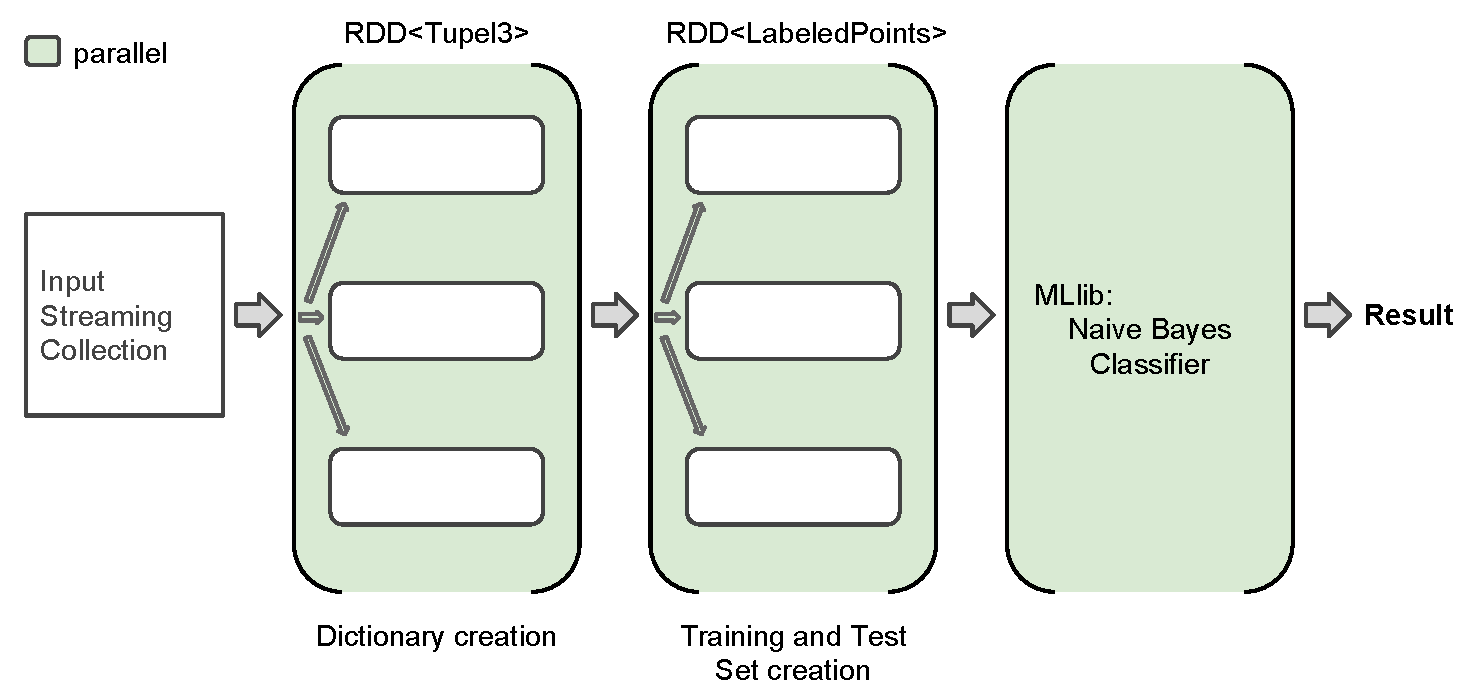
\includegraphics[scale=0.56]{VisualisationOfflineWorkflow.pdf}
  \caption{Offline Workflow}
\end{figure}

\subsection{Evaluation}
%write here
texttexttext

\subsection{Results}
%write here
texttexttext

\subsection{Summary}
%write here
texttexttext




\newpage
\medskip
\bibliography{literatureDB}
\end{document}
